% Канонический TikZ-рисунок варианта 12. Править только здесь.
\long\def\figStereoV12{%
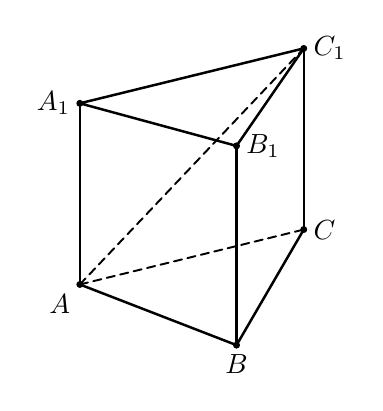
\begin{tikzpicture}[
    x={(1cm,0cm)},
    y={(0.85cm,0.35cm)},
    z={(0cm,1cm)},
    scale=1.15,
    line cap=round,
    line join=round,
    visible/.style={line width=0.9pt},
    hidden/.style={line width=0.7pt,dashed,dash pattern=on 3pt off 2pt}
]

% -------------------------------------------------
% Вершины призмы
% Нижнее основание ABC
% Верхнее основание A1B1C1
% Все рёбра равны 2
% -------------------------------------------------

\coordinate (A)  at (0,0,0);
\coordinate (B)  at (1.9,-0.2,-0.6);
\coordinate (C)  at (1,{sqrt(3)},0);

\coordinate (A1) at (0,0,2);
\coordinate (B1) at (1.9,-0.2,1.6);
\coordinate (C1) at (1,{sqrt(3)},2);

% -------------------------------------------------
% Основания призмы
% -------------------------------------------------


\draw[hidden] (A)--(C);
\draw[visible] (B)--(C);
\draw[visible] (B)--(A);
\draw[visible] (A1)--(B1)--(C1)--cycle;

% -------------------------------------------------
% Боковые рёбра
% -------------------------------------------------

\draw[visible] (A)--(A1);
\draw[visible] (B)--(B1);
\draw[visible] (C)--(C1);

% -------------------------------------------------
% Нужные прямые
% -------------------------------------------------

% BB1 уже является боковым ребром
\draw[hidden] (A)--(C1);

% -------------------------------------------------
% Подписи вершин
% -------------------------------------------------

\fill (A)  circle (1.1pt) node[below left]  {$A$};
\fill (B)  circle (1.1pt) node[below]       {$B$};
\fill (C)  circle (1.1pt) node[right]       {$C$};

\fill (A1) circle (1.1pt) node[left]        {$A_1$};
\fill (B1) circle (1.1pt) node[right]       {$B_1$};
\fill (C1) circle (1.1pt) node[right]       {$C_1$};

\end{tikzpicture}
}
